\chapter{User Interface Design}
Since the mockups of the user interface have already been presented in the RASD document, we will not repeat them here. Instead, we will present the UX diagram

\begin{figure}[H]
    \centering
    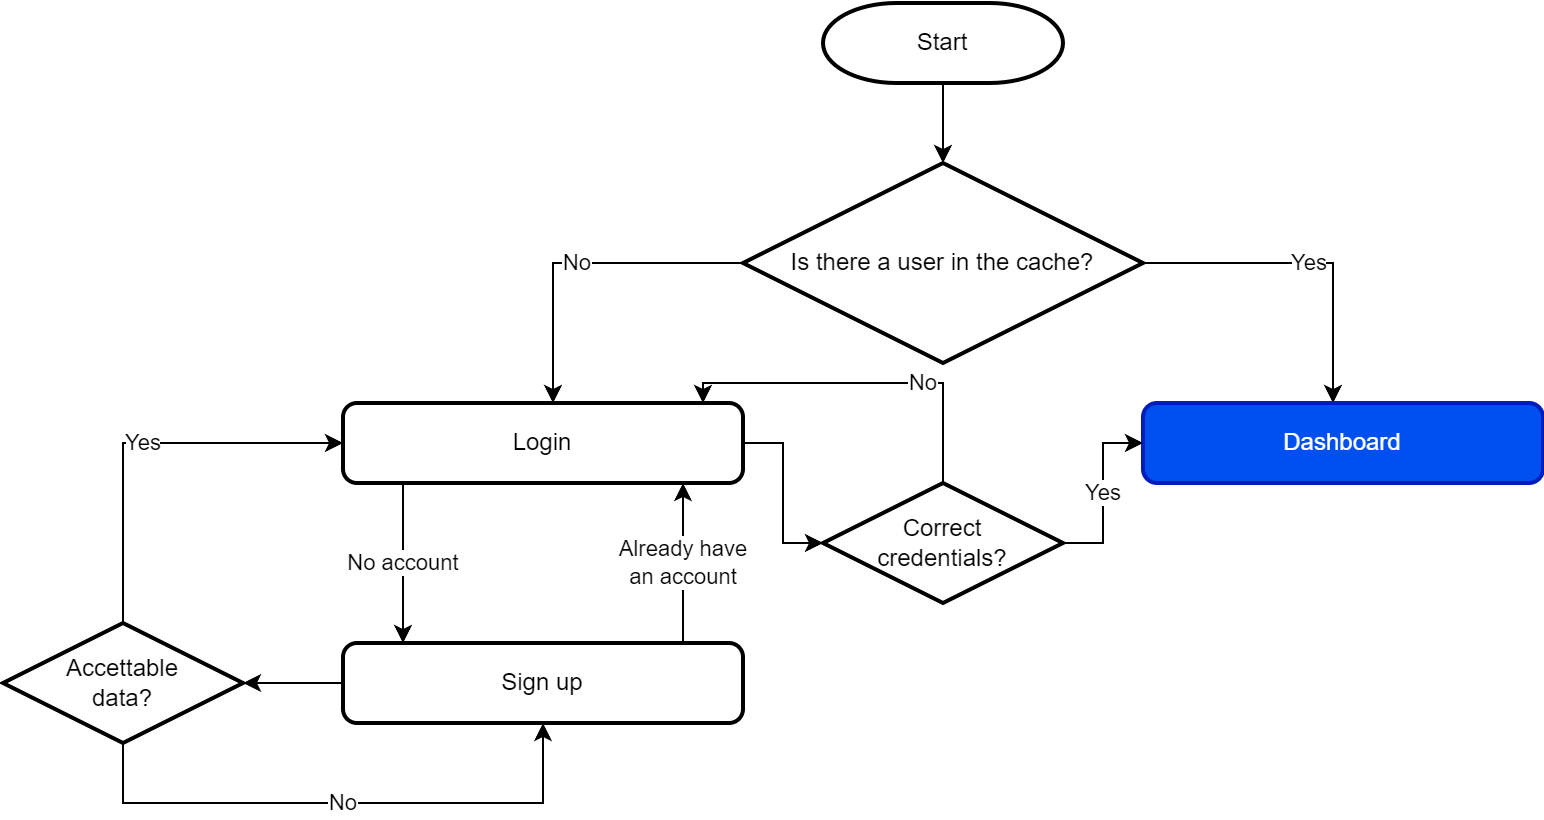
\includegraphics[width=\textwidth]{images/UX/UX-Entry_point.drawio.png}
    \caption{Undifferentiated: Entriy point i.e. the login page}
\end{figure}

\begin{figure}[H]
    \centering
    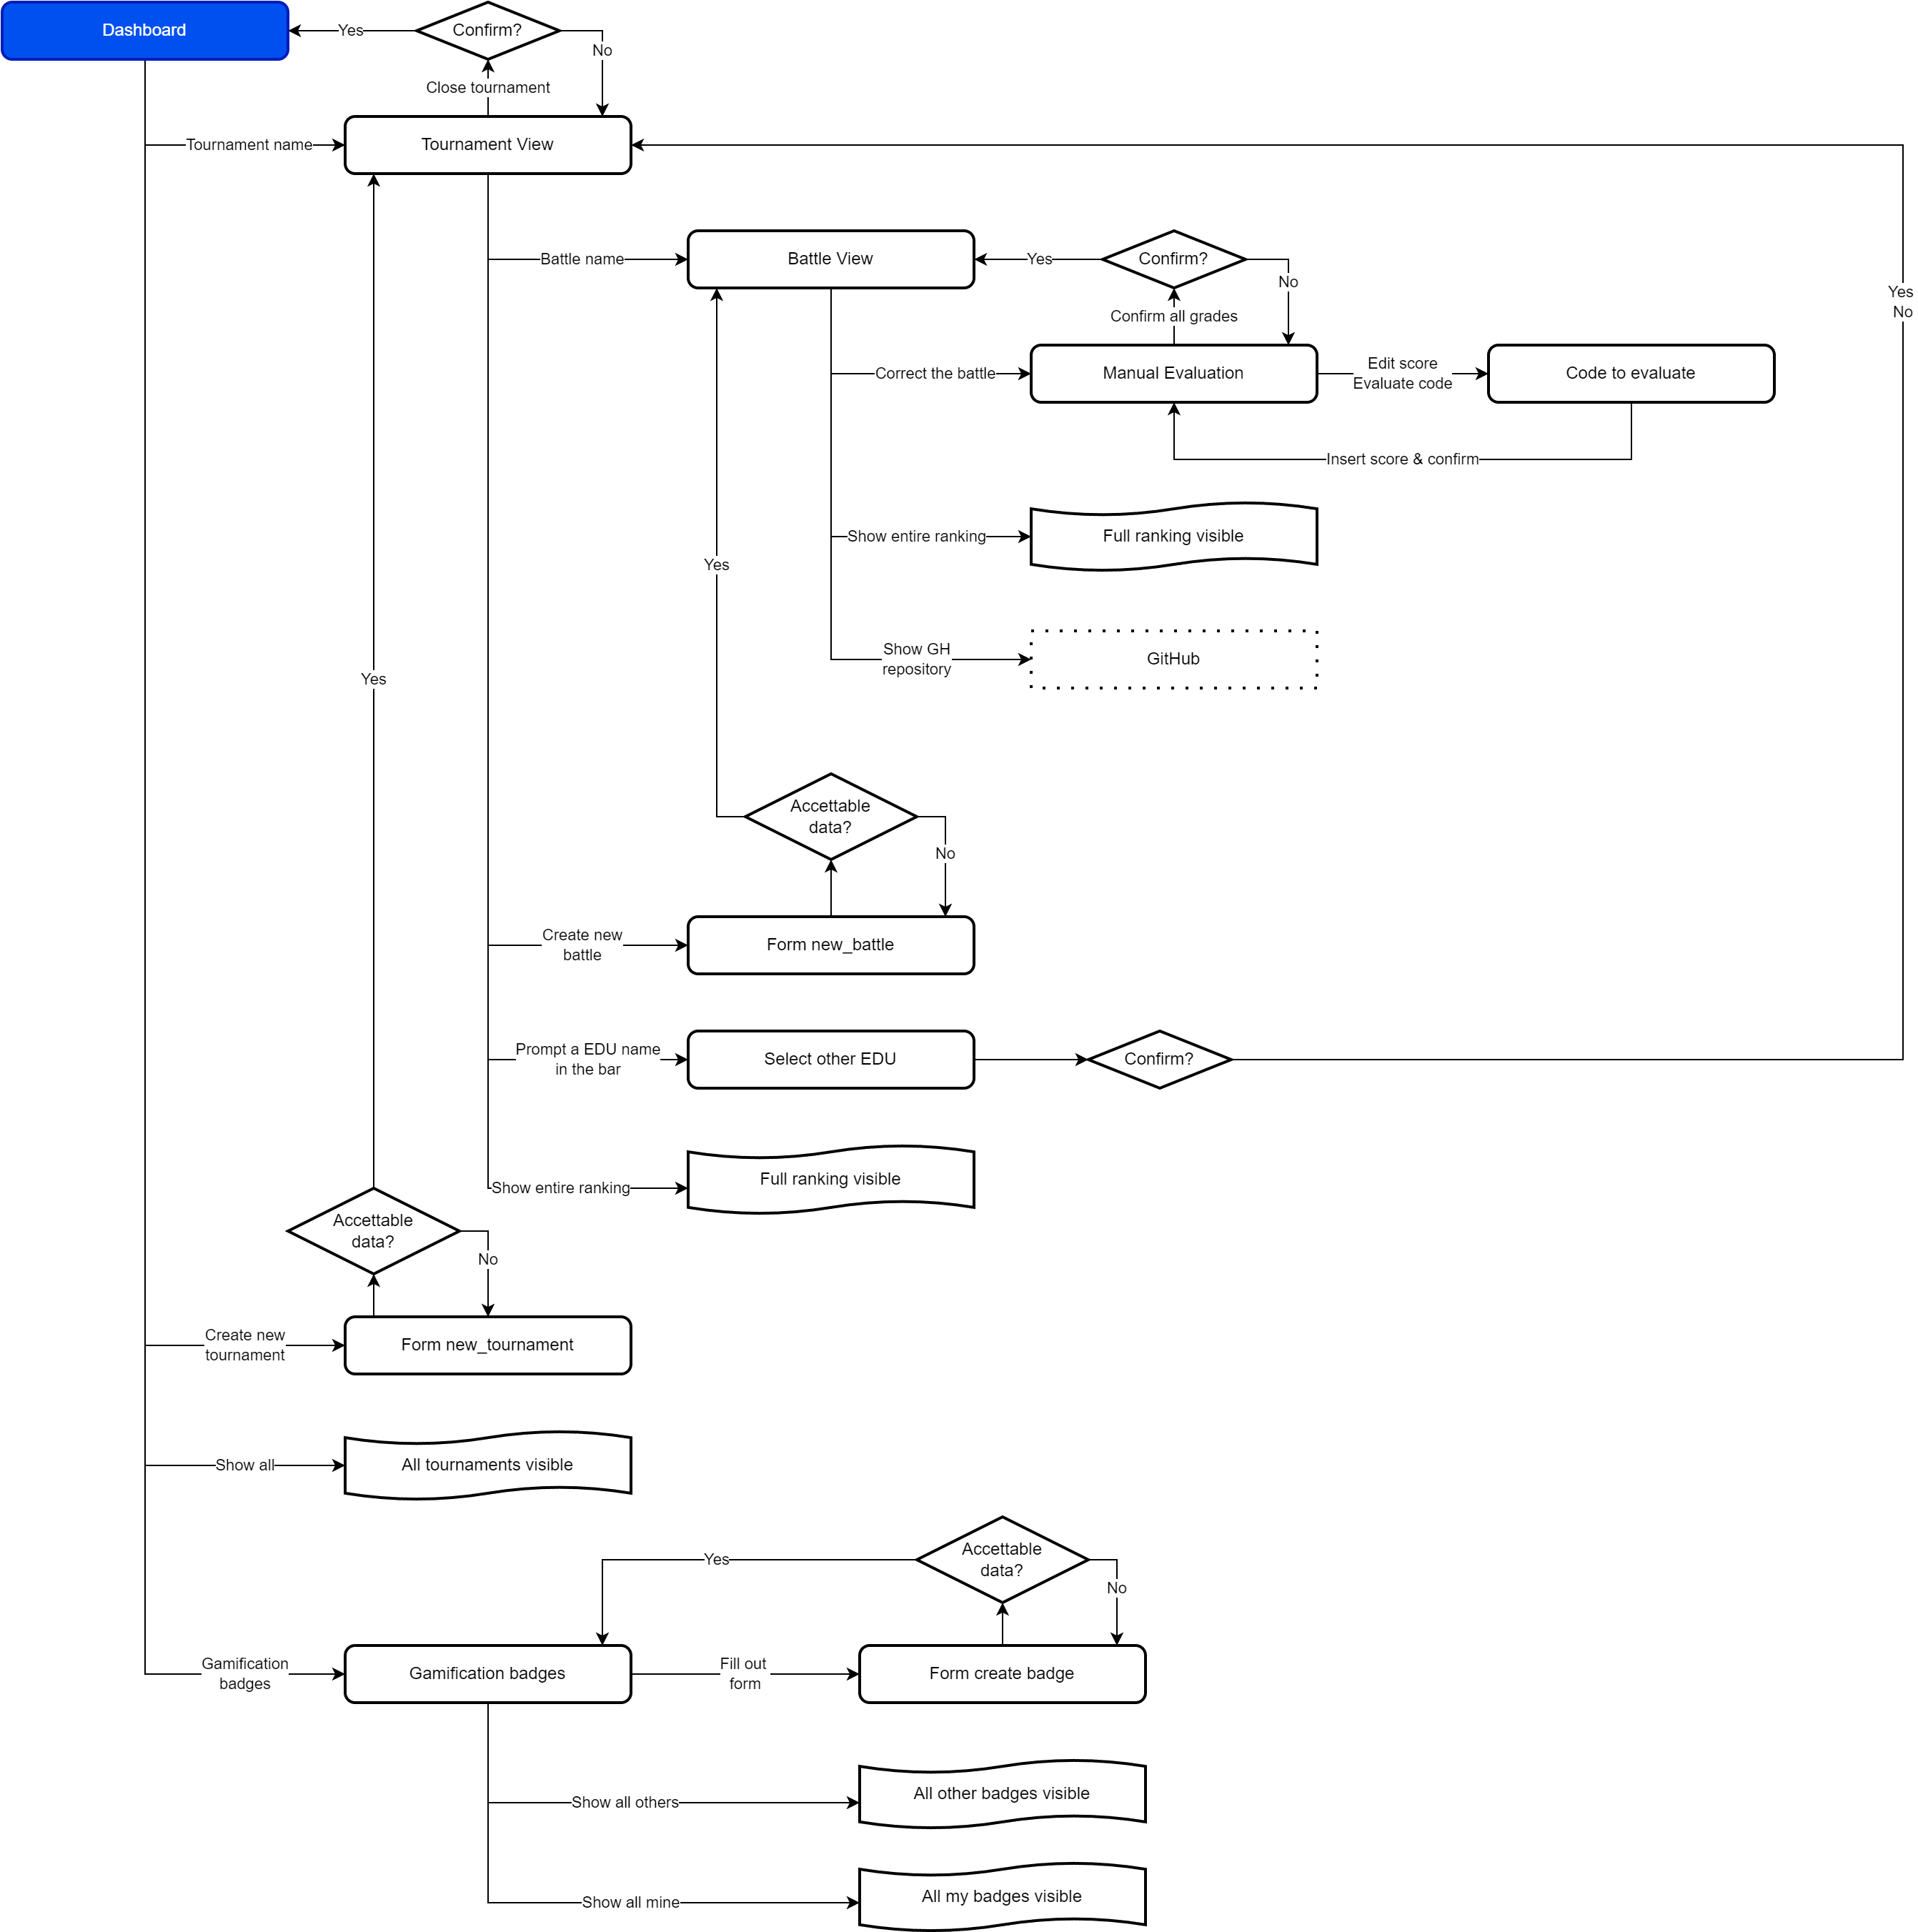
\includegraphics[width=\textwidth]{images/UX/UX-EDU.drawio.png}
    \caption{Flow graph for the EDU}
\end{figure}

\begin{figure}[H]
    \centering
    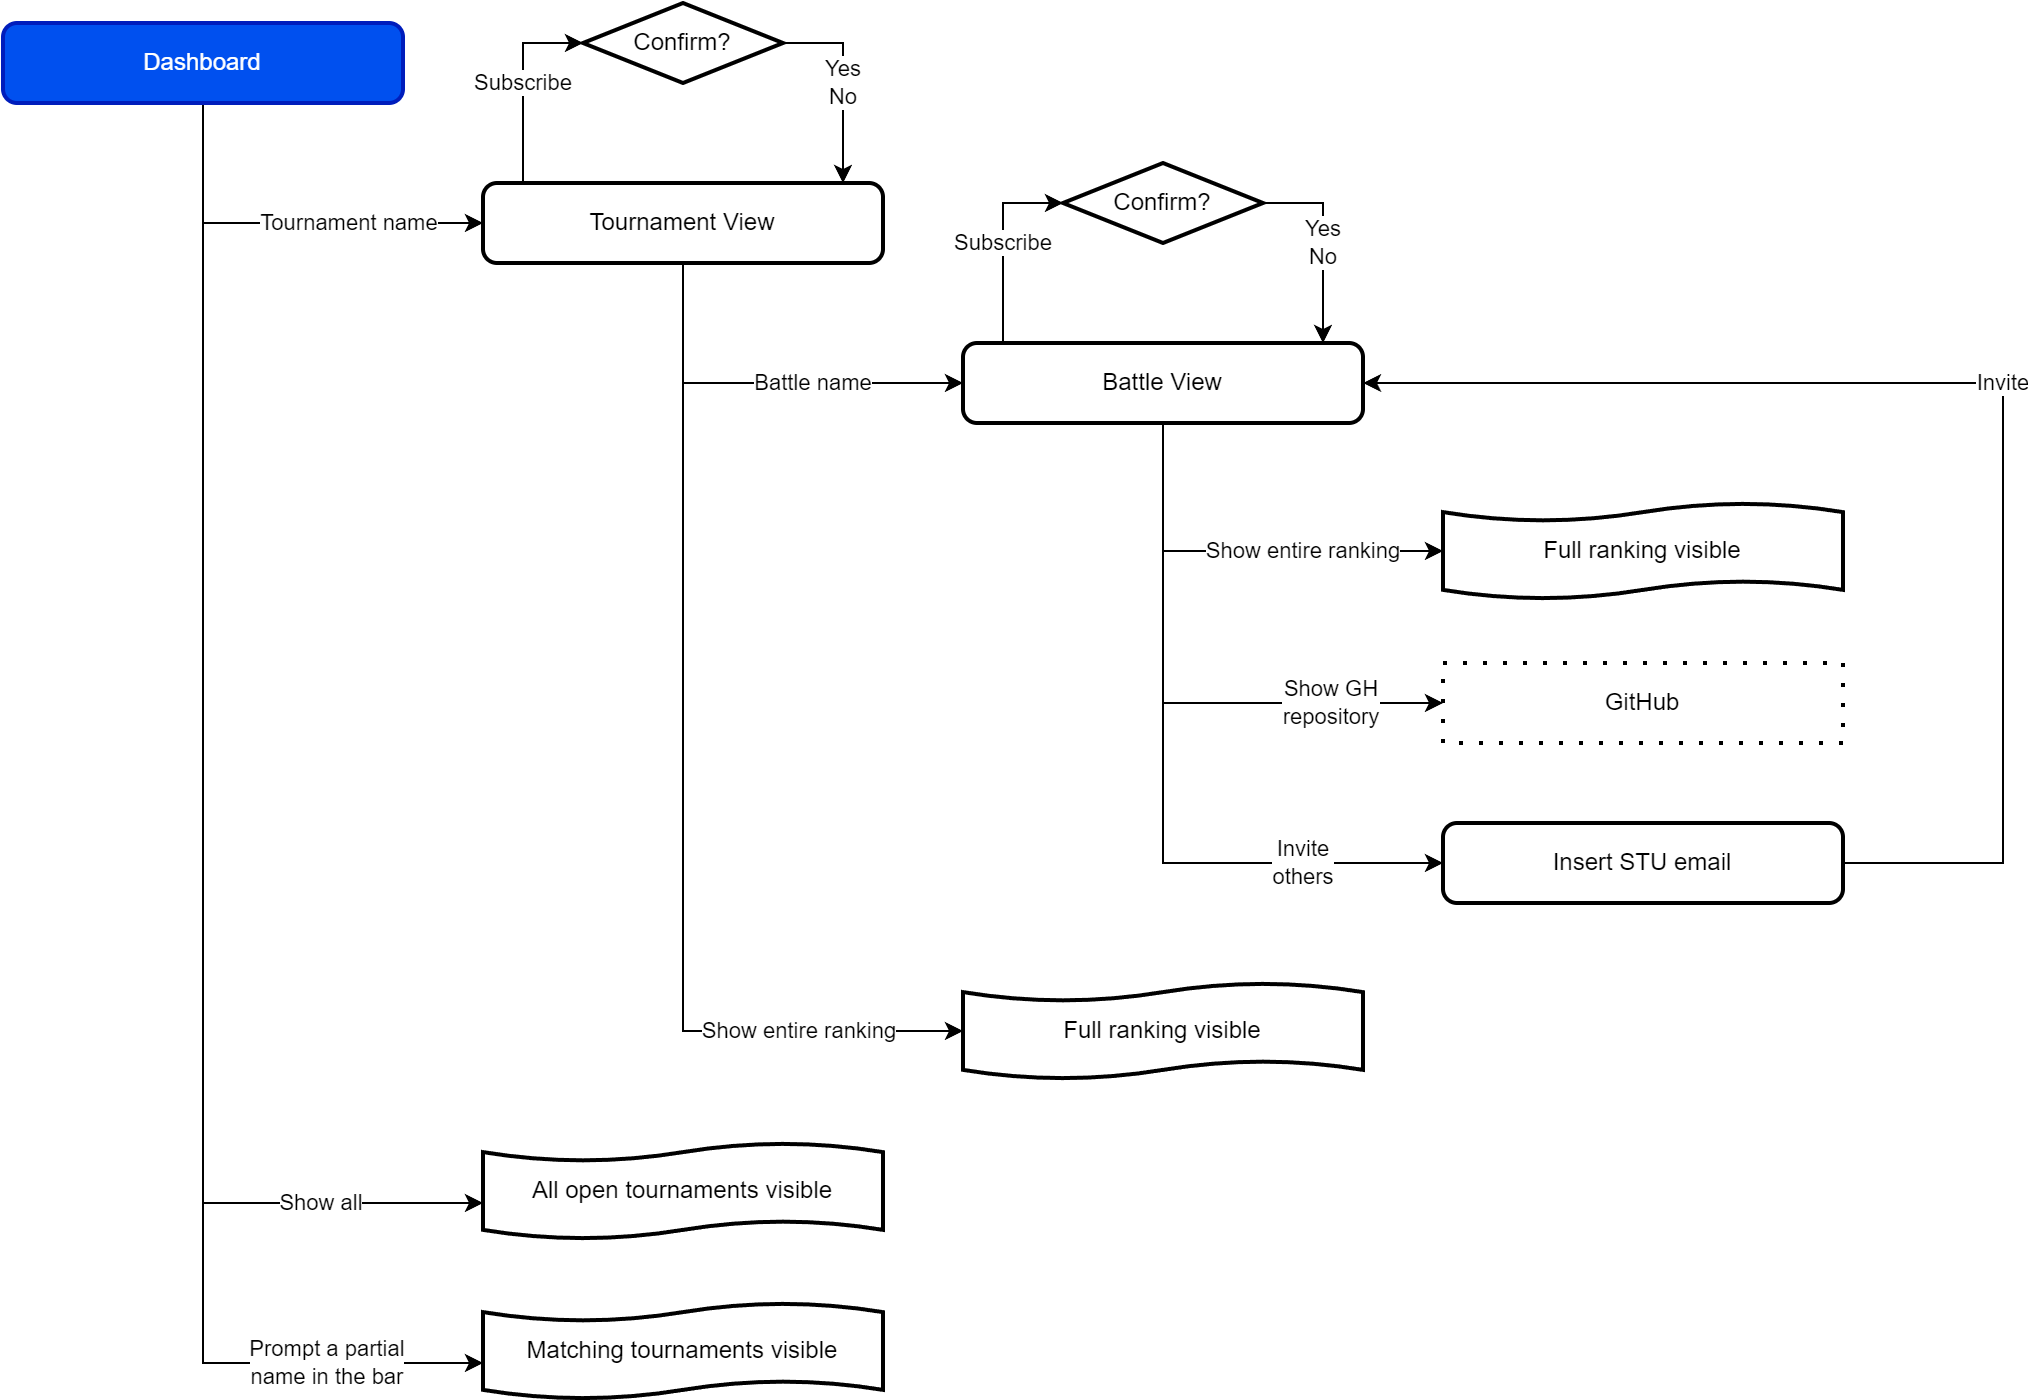
\includegraphics[width=\textwidth]{images/UX/UX-STU.drawio.png}
    \caption{Flow graph for the STU}
\end{figure}

\begin{figure}[H]
    \centering
    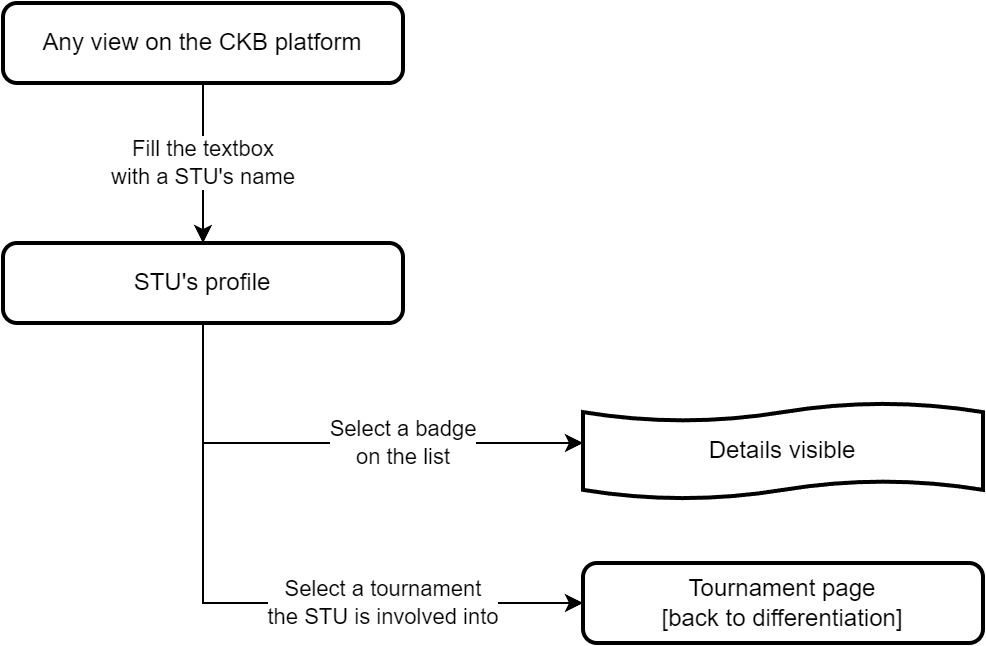
\includegraphics[width=\textwidth]{images/UX/UX-STU_profile.drawio.png}
    \caption{Undifferentiated: viewing a STU's profile}
\end{figure}